%!TEX program = xelatex
\documentclass[aspectratio=169]{beamer}
\usepackage[UTF8]{ctex} % Use default font set
\usepackage{hyperref}

% other packages
\usepackage{latexsym,amsmath,xcolor,multicol,booktabs,calligra}
\usepackage[table]{xcolor}
\usepackage{siunitx} % For \SI command
\usepackage{graphicx,pstricks,listings,stackengine}
\usepackage{tikz}
\usetikzlibrary{patterns}
\usepackage{tikz-3dplot}
\usepackage{fontawesome5}

\author{Yu Shu \& Chihao Shi}
\title{力学A(PHYS1001A.04):刚体部分习题课}
\subtitle{Course NOT easy: The Survival Guide 8, Just Roll With It}
\institute{School of Physics, USTC}
\date{Dec.15, 2025}
\usepackage{USTC} 

% defs
\def\cmd#1{\texttt{\color{red}\footnotesize $\backslash$#1}}
\def\env#1{\texttt{\color{blue}\footnotesize #1}}
\definecolor{deepblue}{rgb}{0,0,0.5}
\definecolor{deepred}{rgb}{0.6,0,0}
\definecolor{deepgreen}{rgb}{0,0.5,0}
\definecolor{halfgray}{gray}{0.55}

\lstset{
    basicstyle=\ttfamily\small,
    keywordstyle=\bfseries\color{deepblue},
    emphstyle=\ttfamily\color{deepred},    % Custom highlighting style
    stringstyle=\color{deepgreen},
    numbers=left,
    numberstyle=\small\color{halfgray},
    rulesepcolor=\color{red!20!green!20!blue!20},
    frame=shadowbox,
}

\begin{document}

\begin{frame}
    \titlepage
    \begin{figure}[htpb]
        \begin{center}
            \includegraphics[width=0.15\linewidth]{pic/ustc_logo_fig-eps-converted-to.pdf}
        \end{center}
    \end{figure}
\end{frame}

\begin{frame}
    \tableofcontents[sectionstyle=show,subsectionstyle=show/shaded/hide,subsubsectionstyle=show/shaded/hide]
\end{frame}

\section{内容回顾与补充拓展}

\subsection{刚体运动学}

\begin{frame}{刚体的核心约束}
    \begin{block}{定义}
        刚体是任意两质点间距离保持恒定的质点系。
        \begin{equation}
            |\vec{r}_i - \vec{r}_j|^2 = C_{ij} \quad (\text{Const})
        \end{equation}
    \end{block}

    \vspace{0.5em}

    \begin{columns}
        \column{0.55\textwidth}
            \textbf{速度场推论:}
            对时间求导,得到刚体运动学的根本判据:
            \begin{equation}
                (\vec{v}_i - \vec{v}_j) \cdot (\vec{r}_i - \vec{r}_j) = 0
            \end{equation}
            \small
            这意味着:刚体上任意两点的\textbf{相对速度},必须\textbf{垂直}于它们的连线。
        
        \column{0.4\textwidth}
            \begin{alertblock}{物理直觉}
                刚体 = 彻底冻结变形的流体。
                \begin{itemize}
                    \item $\nabla \cdot \vec{v} = 0$ (不可压缩)
                    \item 无剪切形变
                \end{itemize}
            \end{alertblock}
    \end{columns}
\end{frame}

\begin{frame}{自由度 (Degrees of Freedom)}
    \textbf{从 $3N$ 到有限个自由度的收敛:}

    \begin{table}
        \centering
        \renewcommand{\arraystretch}{1.3}
        \begin{tabular}{l | c | l}
            \hline
            \textbf{运动类型} & \textbf{DOF} & \textbf{独立坐标示例} \\
            \hline
            \rowcolor{blue!10} 自由刚体 (3D) & \textbf{6} & $x_c, y_c, z_c$ (平动) + 3个欧拉角 (转动) \\
            定点运动 (Fixed Point) & \textbf{3} & $\psi, \theta, \phi$ (欧拉角) \\
            \rowcolor{green!10} 平面平行运动 (Planar) & \textbf{3} & $x, y$ (基点) + $\theta$ (转角) \\
            定轴转动 (Fixed Axis) & \textbf{1} & $\theta$ (转角) \\
            \hline
        \end{tabular}
    \end{table}

    \vspace{0.5em}
    \begin{exampleblock}{思考}
        如果你算出的未知数个数 > DOF,说明你可能遗漏了某些几何约束方程(如纯滚动条件)。
    \end{exampleblock}
\end{frame}

\begin{frame}[shrink=10]{刚体的坐标系:欧拉角}
    \begin{columns}
        \column{0.55\textwidth}
            \textbf{描述定点转动的三个独立变量}:
            将固定系 $Oxyz$ 变为固连系 $Ox'y'z'$,需进行三次旋转($Z \to X \to Z$ 顺规)。
            
            \begin{itemize}
                \item \textcolor{red}{\textbf{1. 进动角 (Precession) $\alpha$}}
                \begin{itemize} \footnotesize
                    \item 绕固定轴 $z$ 旋转。
                    \item 决定了 \textbf{节线 $ON$} (Line of Nodes) 的位置。
                \end{itemize}
                
                \item \textcolor{blue}{\textbf{2. 章动角 (Nutation) $\beta$}}
                \begin{itemize} \footnotesize
                    \item 绕节线 $ON$ 旋转。
                    \item 决定了自转轴 $z'$ 与固定轴 $z$ 的夹角。
                \end{itemize}
                
                \item \textcolor{green!60!black}{\textbf{3. 自转角 (Spin) $\gamma$}}
                \begin{itemize} \footnotesize
                    \item 绕固连轴 $z'$ 旋转。
                    \item 决定了刚体绕自身轴的转动。
                \end{itemize}
            \end{itemize}

            \begin{block}{角速度合成公式}
                $$ \vec{\omega} = \dot{\alpha} \vec{k} + \dot{\beta} \vec{n} + \dot{\gamma} \vec{k}' $$
            \end{block}

        \column{0.45\textwidth}
            \centering
            \includegraphics[width=0.8\textwidth]{pic/1.png}
    \end{columns}
\end{frame}

\begin{frame}{角量的矢量性}
    \begin{itemize}
        \item \textbf{有限角位移 $\Delta \vec{\theta}$}:\textcolor{red}{\textbf{不是矢量}}。
        \begin{itemize}
            \item \footnotesize{原因:不满足矢量加法的交换律(先绕X转90度再绕Y转 $\neq$ 反之)。}
        \end{itemize}
        \item \textbf{无限小角位移 $d\vec{\theta}$}:\textcolor{green}{\textbf{是矢量}}。
        \item \textbf{角速度 $\vec{\omega} = d\vec{\theta}/dt$}:\textcolor{green}{\textbf{是矢量}}。
    \end{itemize}

    \vspace{1em}
    \hrule
    \vspace{1em}

    \begin{columns}
        \column{0.6\textwidth}
            \textbf{角速度的“全域性”}:
            对于刚体上任意两点 $A, B$:
            $$ \vec{\omega}_A = \vec{\omega}_B = \vec{\omega}_{\text{body}} $$
        \column{0.4\textwidth}
            \begin{alertblock}{重要概念}
                $\vec{\omega}$ 是一个\textbf{自由矢量},不依附于任何特定点或轴。
            \end{alertblock}
    \end{columns}
\end{frame}

\begin{frame}[shrink=10]{角位移的矢量性证明}
    \textbf{核心判据}:若物理量是矢量,必须满足加法交换律 $\vec{A} + \vec{B} = \vec{B} + \vec{A}$。
    对于转动,对应旋转矩阵的乘法交换律 $R_1 R_2 = R_2 R_1$。

    \vspace{0.5em}
    \small
    设绕两不同轴转动 $\theta_1, \theta_2$,旋转矩阵泰勒展开至二阶 ($S$为反对称生成元矩阵):
    \begin{equation}
        R(\theta) = I + \theta S + \frac{1}{2}\theta^2 S^2 + O(\theta^3) \quad (\text{其中 } \sin\theta \approx \theta, \cos\theta \approx 1 - \theta^2/2)
    \end{equation}

    \begin{columns}
        \column{0.48\textwidth}
        \begin{alertblock}{1. 有限角位移 $\Delta \vec{\theta}$ (不可易)}
            保留二阶项,比较转动顺序:
            \begin{align*}
                R_1 R_2 &\approx I + \theta_1 S_1 + \theta_2 S_2 + \alert{\theta_1 \theta_2 S_1 S_2} \\
                R_2 R_1 &\approx I + \theta_2 S_2 + \theta_1 S_1 + \alert{\theta_2 \theta_1 S_2 S_1}
            \end{align*}
            由于矩阵乘法一般不可交换 ($S_1 S_2 \neq S_2 S_1$),故:
            $$ R_1 R_2 \neq R_2 R_1 \implies \text{非矢量} $$
        \end{alertblock}
        
        \column{0.48\textwidth}
        \begin{exampleblock}{2. 无限小角位移 $d\vec{\theta}$ (可易)}
            令 $\theta \to d\theta$,忽略二阶及高阶无穷小 ($d\theta^2 \approx 0$):
            \begin{align*}
                R_1 R_2 &\approx (I + d\theta_1 S_1)(I + d\theta_2 S_2) \\
                        &\approx I + d\theta_1 S_1 + d\theta_2 S_2 \\
                R_2 R_1 &\approx I + d\theta_2 S_2 + d\theta_1 S_1
            \end{align*}
            显然相等!满足交换律。
            $$ d\vec{\theta} \text{ 是矢量} \implies \vec{\omega} = \frac{d\vec{\theta}}{dt} \text{ 是矢量} $$
        \end{exampleblock}
    \end{columns}
\end{frame}

\begin{frame}{速度场:基点法}
    任选刚体上一点 $A$ 为基点,另一点 $B$ 的速度可分解为:
    
    \begin{equation}
        \vec{v}_B = \underbrace{\vec{v}_A}_{\text{随基点平动}} + \underbrace{\vec{\omega} \times \vec{r}_{AB}}_{\text{绕基点转动}}
    \end{equation}

    \vspace{1em}
    
    \begin{columns}
        \column{0.5\textwidth}
            \textbf{应用场景:}
            \begin{itemize}
                \item 已知铰链点速度
                \item 已知滚动接触点速度
            \end{itemize}
        \column{0.5\textwidth}
            \textbf{几何意义:}
            刚体的平面运动总是可以看作:
            \begin{enumerate}
                \item 随质心的平动
                \item 绕质心的转动
            \end{enumerate}
    \end{columns}
\end{frame}

\begin{frame}{加速度场}
    对速度公式求导,注意 $\vec{r}_{AB}$ 本身也在旋转 ($\frac{d\vec{r}}{dt} = \vec{\omega} \times \vec{r}$)。

    \begin{block}{刚体两点加速度关系}
        \begin{equation}
            \vec{a}_B = \vec{a}_A + \vec{\alpha} \times \vec{r}_{AB} + \alert{\vec{\omega} \times (\vec{\omega} \times \vec{r}_{AB})}
        \end{equation}
    \end{block}

    \begin{itemize}
        \item $\vec{a}_A$:基点加速度(平动贡献)
        \item $\vec{\alpha} \times \vec{r}_{AB}$:\textbf{切向加速度},源于 $\omega$ 大小改变。
        \item $\alert{\vec{\omega} \times (\vec{\omega} \times \vec{r}_{AB})}$:\textbf{法向加速度},源于 $\omega$ 方向改变。
    \end{itemize}

    \vspace{0.5em}
    \begin{alertblock}{Survival Tip}
        90\% 的错误源于漏掉最后一项(法向加速度)。
        在平面运动中,它简化为指向转轴的 $-\omega^2 \vec{r}_{AB}$。
    \end{alertblock}
\end{frame}

\begin{frame}{瞬时速度中心 (Instantaneous Center, ICR)}
    对于平面平行运动,任一瞬时必存在一点 $P$ (可能在刚体延伸面上),使得 $\vec{v}_P = 0$。

    \begin{columns}
        \column{0.5\textwidth}
            \textbf{瞬心法的威力:}
            $$ \vec{v}_{any} = \vec{\omega} \times \vec{r}_{P \to any} $$
            $$ v = \omega \cdot r $$
            \small{将复杂的平面运动瞬间简化为定轴转动。}
        
        \column{0.5\textwidth}
            \textbf{寻找瞬心:}
            \begin{enumerate}
                \item 两点速度垂线的交点。
                \item 纯滚动接触点。
            \end{enumerate}
    \end{columns}

    \vspace{1em}
    \begin{block}{瞬心的加速度陷阱}
        \textbf{瞬心 $P$ 的速度为 0,但加速度 $\vec{a}_P$ 通常不为 0!}
        \\ 它通常指向质心(向心加速度)。
        \\ $\Rightarrow$ \textcolor{red}{严禁在一般情况下对瞬心列 $M_P = J_P \alpha$!} (除非补上惯性力矩)
    \end{block}
\end{frame}

\subsection{刚体定轴转动}

\begin{frame}{转动惯量 $J$:质量的几何化}
    \begin{columns}
        \column{0.5\textwidth}
            \textbf{定义}:
            量度刚体转动惯性大小的物理量。
            \begin{equation}
                J = \int r_{\perp}^2 dm = \int \rho r_{\perp}^2 dV
            \end{equation}
            \footnotesize{注意:$r_{\perp}$ 是质元到\textbf{转轴}的垂直距离。}
            
            \vspace{0.8em}
            \textbf{回转半径}:
            $$ J = m k^2 \Rightarrow k = \sqrt{J/m} $$
            \textit{工程意义:将刚体等效为一个薄圆环。}

        \column{0.5\textwidth}
            \begin{block}{两大核心定理}
                \textbf{1. 平行轴定理}
                $$ J_d = J_c + md^2 $$
                \textcolor{red}{\textbf{陷阱}}:必须有一个轴是通过\textbf{质心(C)}的。不能在任意两轴间直接转换!
                
                \vspace{0.5em}
                \textbf{2. 垂直轴定理}
                $$ J_z = J_x + J_y $$
                \textcolor{red}{\textbf{限制}}:仅适用于\textbf{平面薄板}刚体。
            \end{block}
    \end{columns}
\end{frame}

\begin{frame}{定轴转动定律}
    对于固定轴 $z$,动力学方程为标量形式:
    
    \begin{alertblock}{转动定律}
        \begin{equation}
            M_z = J_z \alpha = J_z \frac{d\omega}{dt}
        \end{equation}
    \end{alertblock}

    \begin{itemize}
        \item $M_z$:外力对转轴的力矩代数和。
        \item $J_z$:刚体绕该轴的转动惯量。
    \end{itemize}

    \vspace{1em}
    \textbf{力偶}
    \begin{itemize}
        \item 定义:大小相等、方向相反、不共线的一对力。
        \item \textbf{性质}:力偶矩 $\vec{M} = \vec{r} \times \vec{F}$ 与参考点位置\textbf{无关}。
        \item \textit{推论}:可以在刚体平面内任意移动力偶,不改变其转动效应。
    \end{itemize}
\end{frame}

\begin{frame}{核心难点:$\vec{L}$ 与 $\vec{\omega}$}
    \begin{block}{直觉 vs 现实}
        很多同学认为角动量 $\vec{L} \parallel \vec{\omega}$。
        \textbf{错!} 这仅在转轴是\textbf{惯量主轴}时成立。
    \end{block}

    \vspace{0.5em}
    对于一般定轴转动,角动量矢量分解为:
    \begin{equation}
        \vec{L} = \vec{L}_z + \vec{L}_h
    \end{equation}

    \begin{columns}
        \column{0.5\textwidth}
            \textbf{1. 纵向分量 $\vec{L}_z$}
            \begin{itemize}
                \item 平行于转轴
                \item 大小 $L_z = J_z \omega$
                \item 对应标量方程 $M_z = dL_z/dt$
            \end{itemize}
        
        \column{0.5\textwidth}
            \textbf{2. 横向分量 $\vec{L}_h$}
            \begin{itemize}
                \item 垂直于转轴
                \item 由质量分布的\textbf{不对称性}(惯量积)产生
                \item \alert{随刚体一起旋转!}
            \end{itemize}
    \end{columns}
\end{frame}

\begin{frame}{物理后果:动反力}
    根据角动量定理 $\vec{M}_{ext} = \frac{d\vec{L}}{dt}$:
    
    $$ \frac{d\vec{L}}{dt} = \frac{d}{dt}(\vec{L}_z + \vec{L}_h) = \underbrace{J_z \dot{\omega} \vec{k}}_{\text{改变转速}} + \underbrace{\vec{\omega} \times \vec{L}_h}_{\text{改变方向}} $$

    \begin{alertblock}{即使 $\omega$ 恒定 ($\alpha=0$) ...}
        只要 $\vec{L}_h \neq 0$,就有 $\frac{d\vec{L}}{dt} = \vec{\omega} \times \vec{L}_h \neq 0$。
        \\ 这意味着:\textbf{轴承必须提供一个旋转的力矩}来强制刚体绕轴转动。
    \end{alertblock}

    \vspace{0.5em}
    \textbf{应用场景}:
    \begin{itemize}
        \item \textbf{静平衡}:质心在转轴上(消除重力矩)。
        \item \textbf{动平衡}:转轴是惯量主轴(消除 $\vec{L}_h$,消除轴承震动)。
    \end{itemize}
\end{frame}

\begin{frame}{进阶:惯量张量 (Inertia Tensor)}
    角动量与角速度的线性关系可以用矩阵表达:
    \begin{equation}
        \vec{L} = \mathbf{J} \cdot \vec{\omega} \quad \Rightarrow \quad
        \begin{bmatrix} L_x \\ L_y \\ L_z \end{bmatrix} = 
        \begin{bmatrix} 
            J_{xx} & J_{xy} & J_{xz} \\ 
            J_{yx} & J_{yy} & J_{yz} \\ 
            J_{zx} & J_{zy} & J_{zz} 
        \end{bmatrix}
        \begin{bmatrix} \omega_x \\ \omega_y \\ \omega_z \end{bmatrix}
    \end{equation}

    \begin{itemize}
        \item \textbf{对角元} $J_{xx}$:绕轴转动惯量。
        \item \textbf{非对角元} $J_{xy} = - \int xy dm$:\textbf{惯量积} (Product of Inertia),表征质量分布的不对称性。
    \end{itemize}

    \vspace{0.5em}
    \begin{exampleblock}{主轴定理}
        实对称矩阵 $\mathbf{J}$ 必可对角化。即任何刚体都存在3个正交的主轴,绕主轴转动时 $\vec{L} \parallel \vec{\omega}$。
    \end{exampleblock}
\end{frame}

\begin{frame}[shrink=10]{经典模型 A:带质量滑轮的阿特伍德机}
    \begin{columns}
        \column{0.6\textwidth}
        \textbf{场景}:滑轮质量 $M$,半径 $R$,转动惯量 $J$。悬挂质量 $m_1 > m_2$。绳索不可伸长且无相对滑动。
        
        \textbf{核心差异}:
        由于滑轮有惯性,驱动它转动需要力矩,因此两边绳子张力不再相等:
        $ \textcolor{red}{T_1 \neq T_2} $

        \textbf{解题方程组}:
        \begin{enumerate}
            \item \textbf{质点动力学} (牛顿第二定律):
            $m_1 g - T_1 = m_1 a$,$T_2 - m_2 g = m_2 a$
            \item \textbf{刚体定轴转动}:
            $ (T_1 - T_2) R = J \alpha $
            \item \textbf{运动学约束} (无滑移):
            $ a = R \alpha $
        \end{enumerate}

        \column{0.4\textwidth}
        \centering
        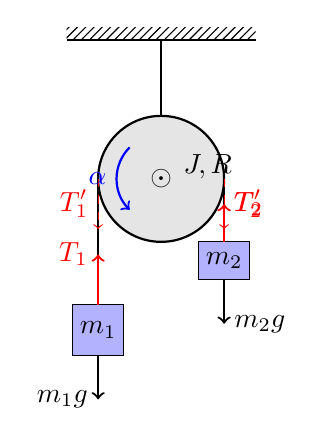
\begin{tikzpicture}[scale=0.8]
            % Ceiling
            \fill [pattern = north east lines] (-1.5, 2.2) rectangle (1.5, 2.4);
            \draw [thick] (-1.5, 2.2) -- (1.5, 2.2);
            \draw [thick] (0, 2.2) -- (0, 0); % Rope holding pulley
            
            % Pulley
            \draw [thick, fill=gray!20] (0,0) circle (1);
            \node at (0,0) {$\odot$};
            \node [right] at (0.2, 0.2) {$J, R$};
            
            % String and Masses
            \draw [thick] (-1, 0) -- (-1, -2);
            \draw [thick] (1, 0) -- (1, -1);
            
            % Mass 1 (Left, Heavier)
            \draw [fill=blue!30] (-1.4, -2.8) rectangle (-0.6, -2);
            \node at (-1, -2.4) {$m_1$};
            \draw [->, thick, red] (-1, -2) -- (-1, -1.2) node[left] {$T_1$};
            \draw [->, thick] (-1, -2.8) -- (-1, -3.5) node[left] {$m_1 g$};
            
            % Mass 2 (Right, Lighter)
            \draw [fill=blue!30] (0.6, -1.6) rectangle (1.4, -1);
            \node at (1, -1.3) {$m_2$};
            \draw [->, thick, red] (1, -1) -- (1, -0.4) node[right] {$T_2$};
            \draw [->, thick] (1, -1.6) -- (1, -2.3) node[right] {$m_2 g$};
            
            % Forces on Pulley (Torque)
            \draw [->, red, dashed] (-1, 0) -- (-1, -0.8) node[midway, left] {$T'_1$};
            \draw [->, red, dashed] (1, 0) -- (1, -0.8) node[midway, right] {$T'_2$};
            
            % Alpha arrow
            \draw [->, thick, blue] (-0.5, 0.5) arc (135:225:0.7) node[midway, left] {$\alpha$};
        \end{tikzpicture}
    \end{columns}
    
    \begin{alertblock}{结论}
        $a = \frac{(m_1 - m_2)g}{m_1 + m_2 + \alert{J/R^2}}$。滑轮的转动惯量等效增加了系统的“惯性质量”。
    \end{alertblock}
\end{frame}

\begin{frame}[shrink=10]{经典模型 B:复摆 (Physical Pendulum)}
    \begin{columns}
        \column{0.55\textwidth}
        \textbf{场景}:刚体绕不通过质心的水平轴 $O$ 转动。质心 $C$ 到轴距离为 $h$。
        
        \textbf{动力学分析}:
        \begin{itemize}
            \item \textbf{重力矩}:$M = -mgh \sin\theta$
            \item \textbf{转动方程}:$J_O \ddot{\theta} = -mgh \sin\theta$
            \item \textbf{微小摆动} ($\sin\theta \approx \theta$):
            $ \ddot{\theta} + \frac{mgh}{J_O} \theta = 0 $
        \end{itemize}
        
        \textbf{关键参数}:
        \begin{itemize}
            \item \textbf{周期}:$T = 2\pi \sqrt{\frac{J_O}{mgh}}$
            \item \textbf{平行轴定理应用}:$J_O = J_C + mh^2$
            \item \textbf{等效摆长}:$l_{eq} = \frac{J_O}{mh} = h + \frac{J_c}{mh}$
        \end{itemize}

        \column{0.45\textwidth}
        \centering
        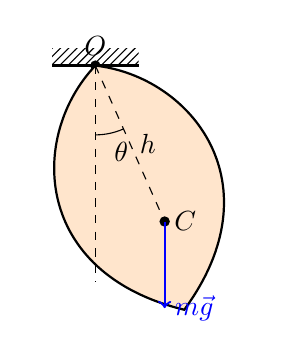
\begin{tikzpicture}[scale=1.1]
            % Pivot
            \fill [pattern = north east lines] (-0.5, 0) rectangle (0.5, 0.2);
            \draw [thick] (-0.5, 0) -- (0.5, 0);
            \fill (0,0) circle (0.06) node[above] {$O$};
            
            % Rigid Body (Potato shape)
            \draw [thick, fill=orange!20, rotate around={20:(0,0)}] 
                (0,0) .. controls (1,-0.5) and (1.5,-2) .. (0,-3) 
                .. controls (-1.5,-2) and (-1,-0.5) .. (0,0);
            
            % Center of Mass
            \coordinate (C) at (0.8, -1.8);
            \fill (C) circle (0.06) node[right] {$C$};
            \draw [dashed] (0,0) -- (C) node[midway, right] {$h$};
            
            % Vertical Line
            \draw [dashed] (0,0) -- (0, -2.5);
            
            % Angle theta
            \draw (0, -0.8) arc (270:294:0.8);
            \node at (0.3, -1) {$\theta$};
            
            % Force mg
            \draw [->, thick, blue] (C) -- ++(0, -1) node[right] {$m\vec{g}$};
            
            % dL/dt indicator (optional)
            %\draw [->, red] (C) -- ++(-0.5, 0) node[left] {$M$};
        \end{tikzpicture}
    \end{columns}

    \begin{exampleblock}{拓展:打击中心 (Center of Percussion)}
        若在 $O$ 点下方距离 $l_{eq}$ 处(打击中心)施加水平冲击,$O$ 点处瞬时无水平反力。
        \small{\textit{应用:棒球棒击球的最佳位置(不震手)。}}
    \end{exampleblock}
\end{frame}

\subsection{刚体的平动}

\begin{frame}{分而治之:运动分解的哲学}
    平面平行运动 = \textbf{随基点的平动} + \textbf{绕基点的转动}。
    
    \begin{block}{为什么永远首选“质心”作为基点?}
        动力学方程中,若选任意点 $A$ 为参考点,力矩方程为:
        $$ \vec{M}_A = \frac{d\vec{L}_A}{dt} + \vec{v}_A \times \vec{P} $$
        只有当 $A$ 点满足以下任一条件时,惯性项 $\vec{v}_A \times \vec{P}$ 消失,方程简化为 $M=J\alpha$:
        \begin{enumerate}
            \item $A$ 是固定点 ($\vec{v}_A = 0$)
            \item $A$ 是质心 ($\vec{v}_A \parallel \vec{P} = m\vec{v}_c$)
            \item $A$ 的加速度指向质心 (特殊情况)
        \end{enumerate}
    \end{block}
\end{frame}

\begin{frame}{标准动力学方程组}
    对于平面平行运动,我们总是列写以下三个独立的标量方程:

    \begin{columns}
        \column{0.5\textwidth}
            \textbf{1. 质心运动定理 (平动)}
            \begin{align}
                \sum F_x &= m a_{cx} \\
                \sum F_y &= m a_{cy}
            \end{align}
            
        \column{0.5\textwidth}
            \textbf{2. 绕质心转动定理 (转动)}
            \begin{equation}
                \sum M_c = J_c \alpha
            \end{equation}
            \small{\textit{注意:此处 $J_c$ 必须是绕质心的转动惯量。}}
    \end{columns}

    \vspace{1em}
    \hrule
    \vspace{1em}

    \textbf{3. 运动学约束}
    \begin{itemize}
        \item 需要寻找 $a_c$ 与 $\alpha$ 之间的几何关系。
        \item 典型约束:纯滚动 $\Rightarrow a_c = R\alpha$。
    \end{itemize}
\end{frame}

\begin{frame}{纯滚动:约束的艺术}
    \begin{block}{定义}
        刚体与接触面之间无相对滑动 $\Rightarrow$ 接触点相对速度为 0。
        $$ v_{\text{contact}} = 0 \implies v_c = R\omega, \quad a_c = R\alpha $$
    \end{block}

    \vspace{0.5em}
    \textbf{静摩擦力的“二律背反”}:
    \begin{itemize}
        \item \textbf{动力学角色}:它是“约束力”(Constraint Force)。
            \begin{itemize}
                \item 大小:\alert{未知!} 由牛顿方程解出,\textbf{绝不是} $\mu N$。
                \item 判据:解出 $f$ 后,若 $f \le \mu_s N$,假设成立;否则打滑。
            \end{itemize}
        \item \textbf{能量角色}:它是“不做功的力”。
            \begin{itemize}
                \item 接触点瞬时位移为 0 $\Rightarrow$ 功率 $P = \vec{f} \cdot \vec{v} = 0$。
                \item 功能:它不消耗机械能,只负责在平动能和转动能之间进行转化。
            \end{itemize}
    \end{itemize}
\end{frame}

\begin{frame}{Survival Skill:摩擦力方向怎么判?}
    \begin{exampleblock}{场景:轮子受外力 $F$ 作用}
        摩擦力方向并不总是阻碍运动,它阻碍的是“相对滑动的趋势”。
    \end{exampleblock}

    \begin{columns}
        \column{0.5\textwidth}
            \textbf{方法一:物理直觉法}
            \begin{enumerate}
                \item 假设地面光滑 ($\mu=0$)。
                \item 分析接触点 $P$ 的加速度 $a_P = a_c - R\alpha$ 的方向。
                \item 摩擦力方向与 $a_P$ 相反。
            \end{enumerate}
        
        \column{0.5\textwidth}
            \textbf{方法二:代数法}
            \begin{enumerate}
                \item 永远假设摩擦力 $f$ 指向正方向 (如向右)。
                \item 列方程:$F+f=ma_c$, $FR-fR=J\alpha$。
                \item 解出 $f$。
                \item 若 $f>0$,方向正确;若 $f<0$,方向反向。
            \end{enumerate}
    \end{columns}
\end{frame}

\begin{frame}{滚动摩阻:不是力,是力矩}
    \begin{columns}
        \column{0.6\textwidth}
            \textbf{现象}:
            即使是纯滚动,物体最终也会停下来。静摩擦力不做功,那能量去哪了?
            
            \vspace{0.5em}
            \textbf{机制}:
            \begin{itemize}
                \item 刚体/地面发生微小形变。
                \item 支持力 $F_N$ 分布不均,合力作用点向前偏移距离 $\delta$。
                \item 产生阻碍转动的力偶矩:
            \end{itemize}
            \begin{equation}
                M_f = F_N \cdot \delta
            \end{equation}

        \column{0.4\textwidth}
            \centering
            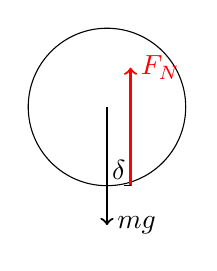
\begin{tikzpicture}
                \draw (0,0) circle (1);
                \draw[->, thick] (0,0) -- (0,-1.5) node[right] {$mg$};
                \draw[->, thick, red] (0.3,-1) -- (0.3,0.5) node[right] {$F_N$};
                \draw[dashed] (0,-1) -- (0.3,-1);
                \node at (0.15, -0.8) {$\delta$};
            \end{tikzpicture}
    \end{columns}
    
    \vspace{0.5em}
    \footnotesize{$\delta$ 称为滚动摩阻系数(长度量纲)。通常 $\delta \ll R$,所以滚动比滑动省力得多。}
\end{frame}

\begin{frame}{瞬心法动力学的雷区}
    我们知道瞬心 $P$ 处速度 $v_P=0$,那么能否直接写 $M_P = J_P \alpha$?

    \pause
    \begin{alertblock}{一般情况:NO!}
        对任意动点 $A$ 的力矩方程为:
        $$ \vec{M}_A = J_A \vec{\alpha} + \vec{r}_{AC} \times m \vec{a}_A $$
        瞬心 $P$ 的加速度 $\vec{a}_P$ 通常指向质心 (向心加速度 $R\omega^2$),不为零!
    \end{alertblock}

    \pause
    \textbf{特例豁免 (The Loophole)}:
    对于\textbf{圆柱/球体做纯滚动}:
    \begin{itemize}
        \item 瞬心 $P$ 为接触点。
        \item $\vec{a}_P$ 指向圆心 $C$ (质心)。
        \item 位置矢量 $\vec{r}_{PC}$ 与 $\vec{a}_P$ 平行 $\Rightarrow$ 叉乘项为 0。
    \end{itemize}
    \textcolor{green}{\textbf{只有在这种几何对称且纯滚动的特例下}},才可以直接用 $M_P = J_P \alpha$ (其中 $J_P = J_c + mR^2$)。
\end{frame}

\begin{frame}{刚体平动解题决策树}
    拿到一个刚体平面运动问题:

    \begin{enumerate}
        \item \textbf{问什么?}
        \begin{itemize}
            \item 求速度/角速度/位移 $\to$ \textbf{能量法}。
            \item 求加速度/力/摩擦力 $\to$ \textbf{动力学方程组}。
        \end{itemize}
        
        \item \textbf{摩擦力怎么处理?}
        \begin{itemize}
            \item 题目说“纯滚动” $\to$ 设静摩擦力 $f$ 为未知数,列 $a=R\alpha$。
            \item 题目说“打滑/光滑” $\to$ $f = \mu N$ 或 $f=0$,无运动学约束。
            \item 临界状态 $\to$ 先按纯滚动算,看算出的 $f$ 是否大于 $\mu N$。
        \end{itemize}

        \item \textbf{方程怎么列?}
        \begin{itemize}
            \item 质心平动 + 绕质心转动。
            \item (仅限纯滚圆轮)绕接触点转动 ($M_P = J_P \alpha$)。
        \end{itemize}
    \end{enumerate}
\end{frame}

\subsection{刚体的能量}

\begin{frame}{能量法的重要作用 (Why Energy?)}
    \begin{block}{标量的优雅}
        动力学方程 ($\vec{F}=m\vec{a}, \vec{M}=d\vec{L}/dt$) 是矢量微分方程,处理方向变化(如法向加速度)非常繁琐。
        能量法是标量方程,是牛顿定律的\textbf{空间积分}形式。
    \end{block}

    \vspace{1em}
    \begin{columns}
        \column{0.5\textwidth}
            \textbf{何时使用能量法?}
            \begin{itemize}
                \item \textcolor{green}{\faCheck} 求速率 $v$、角速度 $\omega$
                \item \textcolor{green}{\faCheck} 求位移 $x$、角度 $\theta$
                \item \textcolor{green}{\faCheck} 系统自由度少,约束力不做功
            \end{itemize}
        
        \column{0.5\textwidth}
            \textbf{何时不能用?}
            \begin{itemize}
                \item \textcolor{red}{\faTimes} 求时间 $t$ (除非积分)
                \item \textcolor{red}{\faTimes} 求约束力 $N, f$ (能量把它们“积”没了)
                \item \textcolor{red}{\faTimes} 碰撞瞬间 (需用角动量)
            \end{itemize}
    \end{columns}
\end{frame}

\begin{frame}{柯尼希定理:动能的彻底解耦}
    对于平面平行运动,刚体总动能可以无交叉项地分解:

    \begin{alertblock}{König's Theorem}
        \begin{equation}
            E_k = \underbrace{\frac{1}{2} m v_c^2}_{\text{随质心平动}} + \underbrace{\frac{1}{2} J_c \omega^2}_{\text{绕质心转动}}
        \end{equation}
    \end{alertblock}

    \textbf{为什么没有交叉项?}
    $$ E_k = \sum \frac{1}{2} m_i (\vec{v}_c + \vec{v}'_i)^2 = \frac{1}{2} m v_c^2 + \frac{1}{2} \sum m_i {v'_i}^2 + \vec{v}_c \cdot \alert{(\sum m_i \vec{v}'_i)} $$
    在质心系中,总动量 $\sum m_i \vec{v}'_i = 0$,因此交叉项消失。
    
    \begin{exampleblock}{警告 (Warning)}
        此公式仅对\textbf{质心}成立。若选其他基点 $A$,必须加上交叉项,或者使用瞬心法。
    \end{exampleblock}
\end{frame}

\begin{frame}{瞬心法:定轴转动的等效}
    若已知瞬时速度中心 (ICR) $P$,刚体看似绕 $P$ 做定轴转动。
    
    \begin{equation}
        E_k = \frac{1}{2} J_P \omega^2
    \end{equation}

    \begin{columns}
        \column{0.6\textwidth}
            \textbf{这与柯尼希定理矛盾吗?}
            \\ 不矛盾。利用平行轴定理 $J_P = J_c + m d^2$:
            \begin{align*}
                E_k &= \frac{1}{2} (J_c + m d^2) \omega^2 \\
                    &= \frac{1}{2} J_c \omega^2 + \frac{1}{2} m \underbrace{(d\omega)^2}_{v_c^2} \quad \text{(得证)}
            \end{align*}
        
        \column{0.4\textwidth}
            \begin{block}{技巧}
                对于纯滚动轮子,用 $E_k = \frac{1}{2} J_{\text{contact}} \omega^2$ 计算动能通常比拆成两项快一倍。
            \end{block}
    \end{columns}
\end{frame}

\begin{frame}{刚体做功的微观机制}
    $$ dW = \vec{F} \cdot d\vec{r}_A \quad (\text{力作用于A点}) $$
    $$ dW = M_z d\theta \quad (\text{力矩做功}) $$

    \vspace{1em}
    \textbf{1. 内力做功之和为零}
    \begin{itemize}
        \item 刚体任意两点间距不变 $\Rightarrow$ 沿相互作用力方向无相对位移。
        \item \textit{对比}:流体(压缩做功)、弹簧(形变做功)内力做功不为零。
    \end{itemize}

    \vspace{0.5em}
    \textbf{2. 重力的功}
    \begin{itemize}
        \item 无论刚体如何翻滚,重力功只取决于质心高度变化。
        \item $W_g = - \Delta E_p = m g (h_{c1} - h_{c2})$。
    \end{itemize}
\end{frame}

\begin{frame}{The Big Trap: 摩擦力做功吗?}
    \begin{alertblock}{结论先行}
        \begin{itemize}
            \item \textbf{纯滚动}中的静摩擦力:\textbf{不做功}。
            \item \textbf{有滑动}时的动摩擦力:\textbf{做负功}(耗散机械能)。
        \end{itemize}
    \end{alertblock}

    \vspace{1em}
    \textbf{深度解析:为什么静摩擦力不做功?}
    \begin{itemize}
        \item 功率 $P = \vec{f} \cdot \vec{v}_{\text{作用点}}$。
        \item 在纯滚动中,作用点(接触点)是瞬心,其瞬时速度 $\vec{v} = 0$。
        \item $\therefore P = 0 \Rightarrow W = 0$。
    \end{itemize}

    \vspace{0.5em}
    \begin{exampleblock}{物理图像}
        静摩擦力不消耗能量,它只是能量的\textbf{搬运工}:它将轮子的转动动能转化为平动动能(加速过程),或反之。
    \end{exampleblock}
\end{frame}

\begin{frame}{综合应用:杆的滑落 (Slide 82)}
    \textbf{场景}:杆长 $L$,靠墙角静止释放。求脱离墙面时的角度 $\theta$。
    \\ \textit{这是连接能量法与动力学方程的经典桥梁。}

    \pause
    \begin{columns}
        \column{0.5\textwidth}
            \textbf{Step 1: 能量法求速度} (未脱离前)
            $$ mgh = \frac{1}{2} J_{ICR} \omega^2 $$
            利用几何关系求出 $\omega(\theta)$。
            
            \vspace{0.5em}
            \textbf{Step 2: 微分求加速度}
            $$ \alpha = \frac{d\omega}{dt} = \frac{d\omega}{d\theta} \cdot \omega $$
            求出 $\alpha(\theta)$。

        \column{0.5\textwidth}
            \textbf{Step 3: 动力学求力}
            列写水平/垂直方向牛顿方程:
            $$ N_{\text{wall}} = m a_{cx} $$
            需要将 $a_c$ 用 $\alpha, \omega$ 表示。
            
            \vspace{0.5em}
            \textbf{Step 4: 脱离判据}
            令 $N_{\text{wall}} = 0$,解出临界角 $\theta$。
    \end{columns}
\end{frame}

\begin{frame}{能量模块 Survival Guide}
    \begin{enumerate}
        \item \textbf{守恒判据}:
        \begin{itemize}
            \item 只有重力做功 $\to$ 守恒。
            \item 纯滚动 (有摩擦力但无位移) $\to$ 守恒。
            \item 有滑动/空气阻力/轴承摩擦 $\to$ 不守恒 (用功能原理)。
        \end{itemize}
        
        \item \textbf{公式首选}:
        \begin{itemize}
            \item 平面运动一般用柯尼希定理:$E = \frac{1}{2}mv_c^2 + \frac{1}{2}J_c\omega^2$。
            \item 纯转动用:$E = \frac{1}{2}J_{axis}\omega^2$。
        \end{itemize}
        
        \item \textbf{解题流}:
        \begin{itemize}
            \item 问速度/位置 $\to$ 能量法。
            \item 问力/时间 $\to$ 动力学/动量法。
            \item 问变力做功 $\to$ 动能定理。
        \end{itemize}
    \end{enumerate}
\end{frame}

\subsection{刚体的定点运动}

\begin{frame}{定点运动基础:直觉的失效}
    \begin{columns}
        \column{0.6\textwidth}
            \textbf{定义}:刚体上有一点 $O$ 固定不动。
            \begin{itemize}
                \item 自由度:\textbf{3} (欧拉角 $\psi, \theta, \phi$)。
                \item 瞬时轴:刚体绕通过 $O$ 点的瞬时轴转动,但轴的方向在空间和刚体内部都在变化。
            \end{itemize}
            
            \vspace{0.5em}
            \textbf{核心方程}:
            \begin{equation}
                \vec{M}^{ext}_O = \frac{d\vec{L}_O}{dt}
            \end{equation}

        \column{0.4\textwidth}
            \begin{alertblock}{The Tensor Trap}
                在定轴转动中,我们习惯了 $L=J\omega$。
                但在定点运动中:
                $$ \vec{L} = \mathbf{J} \cdot \vec{\omega} $$
                除非绕\textbf{惯量主轴}转动,否则 $\vec{L}$ 与 $\vec{\omega}$ \textbf{不平行}!
            \end{alertblock}
    \end{columns}

    \vspace{1em}
    \small{这意味着:即使没有外力矩 ($\vec{M}=0$),$\vec{L}$ 守恒不代表 $\vec{\omega}$ 恒定(欧拉动力学方程的物理背景)。}
\end{frame}

\begin{frame}{陀螺进动:为什么推不倒?}
    \textbf{场景}:高速旋转的陀螺 ($|\vec{\omega}_s|$ 很大),受重力矩作用。
    
    \begin{columns}
        \column{0.5\textwidth}
            \textbf{直觉预期}:
            重力矩试图让陀螺倒下 ($\theta$ 增大)。
            
            \vspace{0.5em}
            \textbf{实际现象}:
            陀螺不倒,反而绕竖直轴水平旋转 ($\psi$ 变化)。
            \\ $\Rightarrow$ 这就是\textbf{进动 (Precession)}。

        \column{0.5\textwidth}
            \textbf{条件 (规则进动)}:
            $$ \omega_s \gg \Omega $$
            (自转角速度远大于进动角速度)
            \begin{itemize}
                \item 此时可近似认为 $\vec{L} \approx \vec{L}_{spin} \parallel \text{自转轴}$。
                \item 忽略进动本身产生的微小角动量。
            \end{itemize}
    \end{columns}
\end{frame}

\begin{frame}{进动的矢量解析}
    \begin{block}{微分关系}
        $$ \vec{M} = \vec{r}_c \times m\vec{g} $$
        $$ d\vec{L} = \vec{M} dt $$
    \end{block}

    \textbf{几何图像推导}:
    \begin{enumerate}
        \item 重力矩 $\vec{M}$ 水平,垂直于自转轴 $\vec{L}$。
        \item $d\vec{L}$ 的方向与 $\vec{M}$ 相同(水平切向)。
        \item $d\vec{L} \perp \vec{L} \Rightarrow$ \textbf{$\vec{L}$ 的大小不变,只改变方向}。
        \item $\vec{L}$ 的端点在水平面内画圆。
    \end{enumerate}
\end{frame}

\begin{frame}{进动的矢量解析}
    \begin{alertblock}{进动角速度公式}
        由 $\vec{v}_{tip} = \vec{\Omega} \times \vec{r}_{tip}$ 类比:
        $$ \frac{d\vec{L}}{dt} = \vec{\Omega} \times \vec{L} = \vec{M} $$
        大小关系:$M = \Omega L \sin\theta \Rightarrow \Omega = \frac{mgl \sin\theta}{J\omega \sin\theta}$
        \begin{equation}
            \Omega = \frac{mgl}{J\omega}
        \end{equation}
    \end{alertblock}
\end{frame}

\begin{frame}{物理直觉:回转效应 (Gyroscopic Effect)}
    \begin{block}{怎么理解“力矩引起侧向运动”?}
        想象 $\vec{L}$ 是一个有巨大惯性的“流速”。
        \begin{itemize}
            \item 力矩 $\vec{M}$ 像是作用在 $\vec{L}$ 箭头上的横向“推力”。
            \item 当你推一个高速运动的物体(如卫星),它不会立刻沿着推力方向跑,而是轨迹发生偏转。
        \end{itemize}
    \end{block}

    \vspace{1em}
    \textbf{应用实例}:
    \begin{itemize}
        \item \textbf{自行车不倒}:向左倾斜产生向后的力矩 $\to$ 前轮向左进动(转弯)$\to$ 离心力扶正车身。
        \item \textbf{子弹/炮弹}:膛线使弹头旋转,利用进动保持飞行姿态稳定(抗风干扰)。
    \end{itemize}
\end{frame}

\begin{frame}{章动:进动中的“点头”震荡}
    如果初始释放陀螺时,直接松手(初速度为0),它无法直接进入完美的进动状态。

    \begin{columns}
        \column{0.6\textwidth}
            \textbf{能量-动量博弈机制}:
            \begin{enumerate}
                \item \textbf{下落}:重力做功,势能 $\to$ 动能。
                \item \textbf{加速}:获得的动能转化为进动速度 $\Omega$。
                \item \textbf{过冲}:$\Omega$ 增大导致角动量竖直分量 $L_z$ 增加,为了守恒,陀螺必须抬头。
                \item \textbf{减速}:抬头导致势能增加,$\Omega$ 减小,再次下落。
            \end{enumerate}
        
        \column{0.4\textwidth}
            \centering
            \begin{tikzpicture}
                \draw[->] (0,0) -- (0,2) node[above] {$z$};
                \draw[dashed] (0,2) arc (90:30:2 and 0.5);
                \draw[thick, blue, domain=0:4*pi, samples=100] plot ({1.5*cos(\x r)}, {1.5*sin(\x r) + 0.3*cos(3*\x r)});
                \node at (0,-1) {\small 轴心的轨迹(摆线状)};
            \end{tikzpicture}
    \end{columns}

    \vspace{0.5em}
    \begin{exampleblock}{结论}
        章动是能量守恒与角动量守恒相互制约的结果。在有阻尼(摩擦)的情况下,章动会迅速衰减,最终稳定在规则进动。
    \end{exampleblock}
\end{frame}

\begin{frame}{拓展案例:宏观与微观的陀螺}
    \textbf{1. 地球的岁差 (Precession of Equinoxes)}
    \begin{itemize}
        \item \textbf{成因}:地球是椭球体(赤道隆起)。太阳和月球对隆起部分的引力不均匀,产生力矩。
        \item \textbf{结果}:地轴绕黄道极进动,周期约 26,000 年。
        \item \textit{影响:北极星位置改变,春分点西移。}
    \end{itemize}

    \vspace{0.5em}
    \hrule
    \vspace{0.5em}

    \textbf{2. 倒立陀螺 (Tippe Top)}
    \begin{itemize}
        \item \textbf{现象}:陀螺旋转后会自动翻转,柄朝下变为柄朝上,重心升高。
        \item \textbf{解释}:摩擦力矩与角动量的耦合。
        \begin{itemize}
            \item 摩擦力矩试图改变 $\vec{L}$ 的方向。
            \item 陀螺为了保持稳定性,通过翻身来适应新的旋转轴。
            \item \alert{能量来源}:部分转动动能转化为重力势能(总动能减小)。
        \end{itemize}
    \end{itemize}
\end{frame}

\begin{frame}[shrink=10]{宏观案例:地球的岁差 (Precession of Equinoxes)}
    \begin{columns}
        \column{0.55\textwidth}
        \textbf{物理图景}:
        地球并非完美的球体,而是一个赤道略鼓的\textbf{椭球体}。
        
        \vspace{0.5em}
        \textbf{成因机制}:
        \begin{enumerate}
            \item \textbf{姿态}:地轴倾斜 $23.5^\circ$,赤道面与黄道面(公转面)不重合。
            \item \textbf{引力差}:太阳/月球对赤道隆起部分(近端与远端)的引力不等。
            \item \textbf{力矩}:形成一个试图把地轴“扶正”(拉向黄道面法线)的力矩 $\vec{M}$。
        \end{enumerate}

        \vspace{0.5em}
        \begin{alertblock}{结果:进动}
            地轴并没有被“扶正”,而是绕黄道极轴画圆。
            \begin{itemize}
                \item \textbf{周期}:约 25,800 年。
                \item \textbf{后果}:北极星轮换(织女星将来会成为北极星)。
            \end{itemize}
        \end{alertblock}

        \column{0.45\textwidth}
        \centering
        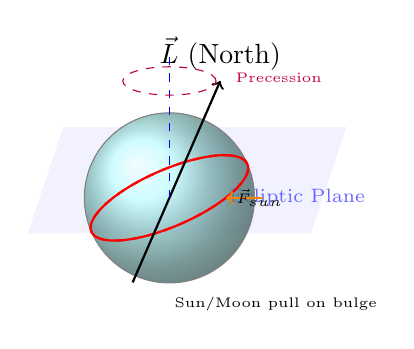
\begin{tikzpicture}[scale=0.9]
            % Ecliptic Plane (Horizontal)
            \fill[blue!10, opacity=0.5] (-2,-0.5) -- (2,-0.5) -- (2.5,1) -- (-1.5,1) -- cycle;
            \node[blue!60, font=\scriptsize] at (1.8, 0) {Ecliptic Plane};
            
            % Earth
            \shade[ball color=cyan!30, opacity=0.8] (0,0) circle (1.2);
            \draw[gray, thin] (0,0) circle (1.2);
            
            % Equator (Bulge) - Tilted
            \draw[red, thick, rotate=23.5] (0,0) ellipse (1.2 and 0.4);
            \draw[red, thick, dashed, rotate=23.5] (0,0) ellipse (1.2 and 0.4); % Back part
            
            % Axis (Spin)
            \draw[->, thick] (0,0) -- ({1.8*sin(23.5)}, {1.8*cos(23.5)}) node[above] {$\vec{L}$ (North)};
            \draw[thick] (0,0) -- ({-1.3*sin(23.5)}, {-1.3*cos(23.5)});
            
            % Ecliptic Pole
            \draw[dashed, blue] (0,0) -- (0, 2);
            
            % Precession Circle
            \draw[->, purple, dashed] (0, 1.65) ellipse ({1.65*sin(23.5)} and 0.2);
            \node[purple, right, font=\tiny] at (0.8, 1.7) {Precession};
            
            % Torque indications (Sun's pull)
            \draw[->, orange, thick] (1.3, 0) -- (0.8, 0) node[right, black, font=\tiny] {$\vec{F}_{sun}$};
            \node[font=\tiny] at (1.5, -1.5) {Sun/Moon pull on bulge};
        \end{tikzpicture}
    \end{columns}
\end{frame}

\begin{frame}[shrink=10]{微观案例:倒立陀螺 (Tippe Top)}
    \begin{columns}
        \column{0.6\textwidth}
        \textbf{现象}:
        一个半球形的陀螺,旋转后会自动翻转,最终以柄为轴旋转,且\textbf{重心升高}。
        
        \vspace{0.8em}
        \textbf{深度解析}:
        这是摩擦力矩与角动量耦合的经典非线性问题。
        \begin{itemize}
            \item \textbf{滑动摩擦}:陀螺接触点存在滑动,摩擦力产生力矩 $\vec{M}_f$。
            \item \textbf{进动效应}:$\vec{M}_f$ 使得角动量 $\vec{L}$ 的方向发生改变(向下翻转)。
            \item \textbf{能量来源}:为什么重心能升高?
            $$ E_{\text{total}} = E_{\text{rot}} + mgh $$
            系统的\textbf{转动动能}通过摩擦耗散,一部分转化为热能,另一部分“泵”入势能,使重心升高。
        \end{itemize}

        \column{0.4\textwidth}
        \centering
        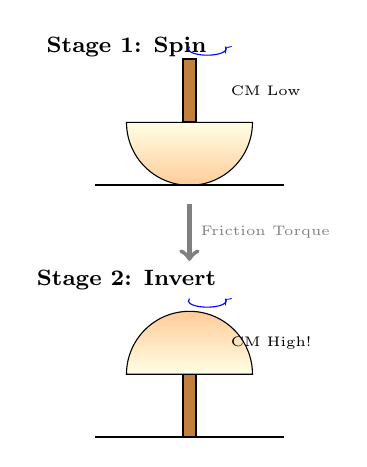
\begin{tikzpicture}[scale=0.8]
            % --- Phase 1: Normal ---
            \begin{scope}[shift={(0,2.5)}]
                \node[font=\footnotesize] at (0, 1.2) {\textbf{Stage 1: Spin}};
                % Body
                \shade[bottom color=orange!40, top color=yellow!10] (0,0) arc (180:360:1) -- cycle;
                \draw (0,0) arc (180:360:1) -- cycle;
                % Stem
                \draw[thick, fill=brown] (0.9, 0) rectangle (1.1, 1);
                % Ground
                \draw[thick] (-0.5, -1) -- (2.5, -1);
                % Spin arrow
                \draw[->, blue] (1, 1.2) arc (160:380:0.3 and 0.1);
                \node[right, font=\tiny] at (1.5, 0.5) {CM Low};
            \end{scope}

            % --- Arrow ---
            \draw[->, ultra thick, gray] (1, 1.2) -- (1, 0.3) node[midway, right, font=\tiny] {Friction Torque};

            % --- Phase 2: Inverted ---
            \begin{scope}[shift={(0,-1.5)}]
                \node[font=\footnotesize] at (0, 1.5) {\textbf{Stage 2: Invert}};
                % Ground
                \draw[thick] (-0.5, -1) -- (2.5, -1);
                % Stem (Touching ground)
                \draw[thick, fill=brown] (0.9, -1) rectangle (1.1, 0);
                % Body (Inverted)
                \shade[top color=orange!40, bottom color=yellow!10] (0,0) arc (180:0:1) -- cycle;
                \draw (0,0) arc (180:0:1) -- cycle;
                % Spin arrow
                \draw[->, blue] (1, 1.2) arc (160:380:0.3 and 0.1);
                \node[right, font=\tiny] at (1.5, 0.5) {\alert{CM High!}};
            \end{scope}
        \end{tikzpicture}
    \end{columns}
    
    \vspace{0.5em}
    \begin{block}{关键点}
        $\vec{L}$ 在空间中尽量保持竖直,但刚体本身相对于 $\vec{L}$ 翻了个身。
    \end{block}
\end{frame}

\subsection{总结与解题方法论}

\begin{frame}{The Big Picture}
    刚体力学不是零散公式的堆砌,而是质点系力学在强约束下的投影。

    \begin{columns}
        \column{0.5\textwidth}
            \begin{block}{1. 几何基础}
                \begin{itemize}
                    \item \textbf{约束}:两点间距不变 $\to$ 相对速度 $\perp$ 连线。
                    \item \textbf{描述}:角速度 $\vec{\omega}$ 是全域自由矢量。
                    \item \textbf{惯量}:$J$ (标量) $\to$ $\mathbf{J}$ (张量)。
                \end{itemize}
            \end{block}
            
            \begin{block}{2. 动力学核心}
                \begin{itemize}
                    \item \textbf{定轴}:$M_z = J_z \alpha$ (+ 动反力)。
                    \item \textbf{平面}:$\sum \vec{F} = m\vec{a}_c$ \& $\sum M_c = J_c \alpha$。
                    \item \textbf{定点}:$\vec{M} = d\vec{L}/dt$ (进动)。
                \end{itemize}
            \end{block}

        \column{0.5\textwidth}
            \begin{block}{3. 能量与守恒}
                \begin{itemize}
                    \item \textbf{动能}:柯尼希定理 (分离平动与转动)。
                    \item \textbf{做功}:内力做功为0;纯滚动摩擦力不做功。
                    \item \textbf{守恒}:
                    \begin{itemize}
                        \item $\vec{M}_{ext} = 0 \to \vec{L}$ 守恒。
                        \item $M_{ext, z} = 0 \to L_z$ 守恒。
                    \end{itemize}
                \end{itemize}
            \end{block}
    \end{columns}
\end{frame}

\begin{frame}{Decision Matrix}
    拿到一道题,如何快速锁定解法?

    \begin{table}
        \centering
        \small
        \renewcommand{\arraystretch}{1.5}
        \begin{tabular}{|c|c|c|}
            \hline
            \textbf{已知/求解目标} & \textbf{首选方法} & \textbf{关键公式/注意点} \\
            \hline
            \rowcolor{blue!10} $v, \omega, \theta, x$ (速度/位移) & \textbf{机械能守恒/动能定理} & $W_{nc} = \Delta E_k$ (查摩擦力是否做功) \\
            \hline
            \rowcolor{green!10} $a, \alpha, t, f, N$ (力/时间) & \textbf{动力学方程组} & $\begin{cases} \vec{F}=m\vec{a}_c \\ M_c = J_c \alpha \end{cases}$ (慎用瞬心力矩) \\
            \hline
            \rowcolor{red!10} 碰撞/打击/角速度突变 & \textbf{角动量(冲量矩)定理} & $\int M dt = \Delta L$ (选定点消除冲力力矩) \\
            \hline
            陀螺/进动 & \textbf{矢量角动量定理} & $\vec{M} = \vec{\Omega} \times \vec{L}$ \\
            \hline
        \end{tabular}
    \end{table}

    \vspace{0.5em}
    \textbf{黄金法则}:
    \begin{itemize}
        \item 看到\textbf{纯滚动} $\to$ 马上写 $v_c = R\omega, a_c = R\alpha$。
        \item 看到\textbf{求极值/脱离} $\to$ 找临界条件 (如 $N=0$ 或 $f = \mu N$)。
    \end{itemize}
\end{frame}

\begin{frame}{综合模型 I:杆的滑落 (The Falling Ladder)}
    \textit{为什么这道题经典?因为它串联了能量、微分运动学和动力学。}

    \begin{columns}
        \column{0.5\textwidth}
            \textbf{题目}:长 $L$ 杆靠墙静止释放,求脱离角 $\theta_d$。
            
            \vspace{0.5em}
            \textbf{解题链条}:
            \begin{enumerate}
                \item \textbf{能量守恒} $\to$ 求 $\omega(\theta)$。
                \item \textbf{运动学求导} $\to$ $\alpha = \omega \frac{d\omega}{d\theta}$ $\to$ 求 $\alpha(\theta)$。
                \item \textbf{质心加速度} $\to$ $\vec{a}_c$ 分解为水平/竖直分量 (需用到 $\omega^2$ 和 $\alpha$)。
                \item \textbf{动力学方程} $\to$ $N_{wall} = m a_{cx}$。
                \item \textbf{临界判据} $\to$ 令 $N_{wall} = 0$,解出 $\theta_d = \arccos(2/3)$。
            \end{enumerate}

        \column{0.5\textwidth}
            \begin{alertblock}{易错点警示}
                \begin{itemize}
                    \item \textbf{瞬心法求动能}:$E_k = \frac{1}{2}J_{ICR}\omega^2$ (快!)。
                    \item \textbf{误区}:脱离时 $N=0$,但这\textbf{不代表}水平加速度为0。脱离瞬间,墙面对杆的约束解除,水平方向力确实消失,但此前积累的速度还在。
                    \item \textbf{质心轨迹}:在脱离前,质心轨迹是圆弧(椭圆规原理);脱离后,质心做抛体运动。
                \end{itemize}
            \end{alertblock}
    \end{columns}
\end{frame}

\begin{frame}{综合模型 II:台球的“滑”与“滚”}
    \textbf{题目}:水平击打半径为 $R$ 的静止台球,击打点高 $h$ (相对球心)。求球何时开始纯滚动?
    
    \vspace{0.5em}
    \textbf{阶段 1:击打瞬间 (Impulse)}
    \begin{itemize}
        \item \textbf{平动}:$F \Delta t = m v_0 \implies v_0 = \frac{I_{imp}}{m}$
        \item \textbf{转动}:$(F \cdot h) \Delta t = J_c \omega_0 \implies \omega_0 = \frac{h I_{imp}}{J_c}$
    \end{itemize}
    
    \begin{exampleblock}{状态分析}
        此时接触点速度 $v_P = v_0 - R\omega_0$。
        \begin{itemize}
            \item 若 $h > J_c/mR$ (击球点很高),$R\omega_0 > v_0$,球会有向后的“回旋”,接触点向前滑。
            \item 若 $h = J_c/mR$ (打击中心),$v_P=0$,\textbf{直接进入纯滚动}!
            \item 若 $h = 0$ (击打中心),$\omega_0=0$,纯滑动。
        \end{itemize}
    \end{exampleblock}
\end{frame}

\begin{frame}{综合模型 II:从滑动到滚动 (Transition)}
    \textbf{阶段 2:滑动过程 (Sliding Phase)}
    假设 $h=0$ (击打中心),则 $v_0 > 0, \omega_0 = 0$。接触点向前滑动。
    \begin{itemize}
        \item \textbf{受力}:动摩擦力 $f_k = \mu mg$ 向后。
        \item \textbf{动力学方程}:
        \begin{align}
            \text{平动减速:} & -\mu mg = m a_c \implies a_c = -\mu g \\
            \text{转动加速:} & \mu mg R = J_c \alpha \implies \alpha = \frac{\mu mg R}{J_c}
        \end{align}
    \end{itemize}
\end{frame}

\begin{frame}{综合模型 II:从滑动到滚动 (Transition)}
    \textbf{阶段 3:临界时刻 (Pure Rolling)}
    $$ v(t) = v_0 - \mu g t, \quad \omega(t) = 0 + \frac{\mu mg R}{J_c} t $$
    当满足 $v(t) = R\omega(t)$ 时,滑动结束,纯滚动开始。
    $$ v_0 - \mu g t = R \left( \frac{\mu mg R}{J_c} t \right) \implies t = \frac{v_0}{\mu g (1 + mR^2/J_c)} $$
    
    \pause
    \small{\textit{结论:对于实心球 ($J_c = \frac{2}{5}mR^2$),最终速度 $v_{final} = \frac{5}{7}v_0$。摩擦力虽然耗散了能量,但也“转换”了动能形式。}}
\end{frame}

\begin{frame}{Must-Check List}
    \begin{enumerate}
        \item \textbf{转动惯量}:
        \begin{itemize}
            \item[$\square$] 这是一个圆盘($1/2$)还是圆环($1$)?
            \item[$\square$] 平行轴定理 $J=J_c+md^2$ 必须从\textbf{质心}出发,不能乱移。
        \end{itemize}
        
        \item \textbf{力矩的正负}:
        \begin{itemize}
            \item[$\square$] 设定逆时针为正后,所有的 $\vec{M}, \vec{\theta}, \vec{\omega}, \vec{\alpha}$ 必须统一符号。
        \end{itemize}
        
        \item \textbf{摩擦力}:
        \begin{itemize}
            \item[$\square$] 看到“纯滚动”,千万别写 $f=\mu N$!它是未知数。
            \item[$\square$] 看到“光滑平面”,意味着 $\alpha=0$ (如果外力过质心),物体只会滑不会转(或匀速转)。
        \end{itemize}
        
        \item \textbf{角动量守恒}:
        \begin{itemize}
            \item[$\square$] 只有合外力矩为0时才守恒。
            \item[$\square$] 注意参考点的选择!碰撞问题通常选\textbf{碰撞接触点}或\textbf{质心}。
        \end{itemize}
        
        \item \textbf{瞬心法}:
        \begin{itemize}
            \item[$\square$] 算动能?大胆用 $E = \frac{1}{2}J_P \omega^2$。
            \item[$\square$] 算力矩?\textbf{住手!} 除非是纯滚圆轮,否则老老实实回质心。
        \end{itemize}
    \end{enumerate}
\end{frame}

\begin{frame}{结语}
    \begin{center}
        \Huge \textbf{Rigid Body Dynamics}
    \end{center}
    
    \vspace{1em}
    \begin{quote}
        "Nature uses only the longest threads to weave her patterns, so that each small piece of her fabric reveals the organization of the entire tapestry." \\
        \hfill --- Richard Feynman
    \end{quote}
    
    \vspace{1em}
    \textbf{核心心法}:
    \begin{itemize}
        \item 几何约束是前提。
        \item 质心分解是通法。
        \item 能量守恒是捷径。
        \item 矢量分析是本质。
    \end{itemize}
    
    \vspace{1em}
    \centerline{\textcolor{blue}{\textbf{祝大家刚体力学满绩!}}}
\end{frame}

\section{作业习题讲解}

\begin{frame}
    \begin{center}
        {\Huge 作业习题讲解}
    \end{center}
\end{frame}

\section{Q\&A}

\begin{frame}
    \begin{center}
        {\Huge\calligra Q\&A}
    \end{center}
\end{frame}

\begin{frame}
    \begin{center}
        {\Huge\calligra Thanks!}
    \end{center}
\end{frame}

\end{document}